% =====================================================================
%          HOW EACH OBJECT IS BUILT (construction drawings)
% =====================================================================
\section{How Each Object Is Built}\label{sec:build}
This section shows the construction of every main object: a side or front drawing (units in metres, as in the code) and a table of its parts, the primitive used for each part and its size and position. All parts are placed with $M=T\,R\,S$ inside the object's own frame (Section~\ref{sec:xf}), so the whole object can then be moved, turned and scaled as one.

\newcommand{\objcard}[3]{\par\medskip\noindent
\begin{minipage}[c]{0.34\textwidth}\centering #2\end{minipage}\hfill
\begin{minipage}[c]{0.63\textwidth}{\color{ramen}\bfseries #1}\par\vspace{1pt}\footnotesize #3\end{minipage}\par\smallskip}
\newcommand{\parts}[1]{\begin{tabular}{@{}p{2.05cm}p{2.25cm}p{5.85cm}@{}}\toprule\textbf{Part}&\textbf{Primitive}&\textbf{Size / placement}\\\midrule #1\bottomrule\end{tabular}}
\tikzset{dim/.style={<->,>={Stealth[length=2.5pt]},gray,thin},
         lbl/.style={font=\tiny,inner sep=1pt}}

\subsection{Shop furniture and food}
\objcard{Ramen bowl (\code{drawRamenBowl}, \code{drawBowl}), drawn at scale 0.24}{%
\begin{tikzpicture}[scale=3.4]
\fill[red!70!black] (-0.22,0) rectangle (0.22,0.06);
\fill[red!75!black] (-0.25,0.06)--(-0.5,0.4)--(0.5,0.4)--(0.25,0.06)--cycle;
\draw[very thick,red!50!black] (-0.51,0.4)--(0.51,0.4);
\draw[dashed,orange] (-0.42,0.29)--(0.42,0.29);
\fill[pink!60!brown] (-0.31,0.41) rectangle (-0.05,0.44);
\fill[white,draw=gray] (0.18,0.43) ellipse (0.08 and 0.035); \fill[yellow!80!orange] (0.18,0.445) ellipse (0.045 and 0.018);
\fill[green!30!black] (-0.04,0.41) -- (0.05,0.41) -- (0.02,0.53) -- (-0.07,0.53) -- cycle;
\draw[dim] (-0.5,-0.07)--(0.5,-0.07) node[midway,below,lbl]{rim \O1.0};
\draw[dim] (0.6,0)--(0.6,0.4) node[midway,right,lbl]{0.40};
\node[lbl,left] at (-0.5,0.29) {broth};
\end{tikzpicture}}{%
\parts{Foot ring & tube & radius 0.22, height 0.06\\
Body & frustum tube & radius $0.25\to0.50$, from $y=0.06$ to $0.40$; red glaze, specular $0.9$, $n=110$\\
Rim & torus & ring radius 0.5, tube 0.015, at $y=0.40$\\
Broth & thin cylinder & \O0.83 at $y=0.29$; specular $(0.9,0.75,0.5)$, $n=85$\\
Noodles & 6 tori + 3 rods & ring radius $0.08\ldots0.28$, tube 0.025\\
Chashu, egg & cylinder; 2 ellipsoids & pork \O0.26; egg white $0.16{\times}0.10{\times}0.20$ with yolk\\
Nori, onion & thin board; 6 tori & nori $0.25{\times}0.3$ tilted $20^\circ$; onion rings radius 0.018\\
Steam & 7 spheres & rising, growing, alpha $0.28\sin\pi\varphi$ (Section~\ref{sec:blend})\\}}

\objcard{Counter stool (\code{drawStool}), six of them}{%
\begin{tikzpicture}[scale=3.4]
\fill[brown!60!black] (-0.18,0) rectangle (0.18,0.04);
\fill[brown!70] (-0.065,0.06)--(-0.055,0.70)--(0.055,0.70)--(0.065,0.06)--cycle;
\fill[brown!50!black] (-0.13,0.35) rectangle (0.13,0.375);
\fill[orange!50!brown] (-0.19,0.70) rectangle (0.19,0.755);
\draw[dim] (0.27,0)--(0.27,0.755) node[midway,right,lbl]{0.755};
\draw[dim] (-0.19,0.81)--(0.19,0.81) node[midway,above,lbl]{seat \O0.38};
\node[lbl,left] at (-0.13,0.36) {ring};
\end{tikzpicture}}{%
\parts{Base disc & cylinder & \O0.36, height 0.04, dark wood\\
Pedestal & frustum & radius $0.065\to0.055$, height 0.64, from $y=0.06$\\
Ring & torus & ring radius 0.13, tube 0.018, at $y=0.36$\\
Seat & cylinder & \O0.38, height 0.055 at $y=0.70$; lacquer $n=55$\\}
The first stool is a selectable object (Tab) and can be moved, rotated and scaled.}

\objcard{Customer table and chair (\code{drawTable}, \code{drawChair})}{%
\begin{tikzpicture}[scale=1.75]
\fill[brown!50] (-0.6,0.69) rectangle (0.6,0.75);
\foreach \x in {-0.52,0.52} \fill[brown!40!black] (\x-0.035,0) rectangle (\x+0.035,0.69);
\draw[dim] (-0.6,0.85)--(0.6,0.85) node[midway,above,lbl]{1.2};
\draw[dim] (-0.72,0)--(-0.72,0.75) node[midway,left,lbl]{0.75};
\begin{scope}[xshift=1.05cm]
\fill[brown!50] (-0.225,0.42) rectangle (0.225,0.47);
\foreach \x in {-0.19,0.19} \fill[brown!40!black] (\x-0.025,0) rectangle (\x+0.025,0.42);
\fill[brown!40!black] (-0.225,0.47) rectangle (-0.175,0.97);
\fill[brown!50] (-0.245,0.85) rectangle (-0.205,1.0);
\node[lbl,below] at (0,-0.02) {chair (side)};
\end{scope}
\end{tikzpicture}}{%
\parts{Table top & textured box & $1.2\times0.06\times0.8$ at $y=0.69$, lacquer $n=55$\\
Table legs & 4 boxes & $0.07\times0.69$ at $(\pm0.52,\pm0.32)$\\
Chair seat & textured box & $0.45\times0.05\times0.45$ at $y=0.42$\\
Backrest & textured box & $0.45\times0.15\times0.04$ at $y=0.85$, $z=-0.2$\\
Legs, back posts & 6 boxes & legs $0.05\times0.42$ at $(\pm0.19,\pm0.19)$; posts $0.05\times0.5$\\}
Placed at scale $0.8\times0.9\times0.8$ (table) and $0.85$ (chairs), with a spot lamp above.}

\objcard{Dining counter (\code{drawCounter}), cross-section}{%
\begin{tikzpicture}[scale=2.2]
\fill[brown!55] (-0.3,0) rectangle (0.3,1.0);
\fill[orange!45!brown] (-0.35,1.0) rectangle (0.45,1.06);
\draw[dim] (-0.3,-0.08)--(0.3,-0.08) node[midway,below,lbl]{0.6};
\draw[dim] (-0.35,1.15)--(0.45,1.15) node[midway,above,lbl]{top 0.8};
\draw[dim] (0.55,0)--(0.55,1.06) node[midway,right,lbl]{1.06};
\node[lbl] at (0,0.5) {body};
\end{tikzpicture}}{%
\parts{Body & textured box & $6.0\times1.0\times0.6$, wood texture, specular $0.65$, $n=40$\\
Top slab & textured box & $6.2\times0.06\times0.8$ at $y=1.0$, shifted $0.05$ toward the stools; lacquer specular $1.0$, $n=60$\\
On top & see bowl, glass & 4 bowls at $x=-2.2+1.5i$, glasses, jars, bottles, glass ball\\}
The lacquered top shows the long Phong highlights of Figure~\ref{fig:phonggouraud}.}

\objcard{Stock pot (\code{drawLargeRamenPot}), two on the stove}{%
\begin{tikzpicture}[scale=3.0]
\fill[gray!60] (-0.30,0)--(-0.32,0.55)--(0.32,0.55)--(0.30,0)--cycle;
\fill[gray!80] (-0.345,0.53) rectangle (0.345,0.575);
\draw[dashed,orange] (-0.29,0.53)--(0.29,0.53);
\foreach \s in {-1,1} {\draw[thick,gray!30!black] (\s*0.40,0.42) circle (0.05); \fill[gray!30!black] (\s*0.34-0.025,0.385) rectangle (\s*0.34+0.025,0.455);}
\draw[dim] (-0.32,0.65)--(0.32,0.65) node[midway,above,lbl]{\O0.64};
\draw[dim] (0.52,0)--(0.52,0.55) node[midway,right,lbl]{0.55};
\end{tikzpicture}}{%
\parts{Vessel & frustum & radius $0.30\to0.32$, height 0.55; steel $(0.42,0.43,0.46)$, specular 1, $n=90$, sphere-map reflection\\
Broth, foam & disc, torus & \O0.58 at $y=0.53$; foam ring radius 0.27\\
Rolled rim & torus & radius 0.32, tube 0.025, $n=120$\\
Handles & 2 tori, plates, rivets & radius 0.07 at $x=\pm0.35$, $y=0.42$\\}
Ray traced with key \code{R} (reflection, Figure~\ref{fig:rt1}).}

\subsection{Lanterns, banner and wind chime}
\objcard{Chochin paper lantern (\code{drawChochinLantern})}{%
\begin{tikzpicture}[scale=2.6]
\draw[thick,yellow!60!brown] (0,0) circle (0.03);
\shade[inner color=yellow!80!orange,outer color=orange!80!red] (0,-0.35) ellipse (0.30 and 0.33);
\foreach \y in {-0.6,-0.52,-0.44,-0.35,-0.26,-0.18,-0.1} \draw[orange!50!black,thin] ({-sqrt(1-((\y+0.35)/0.33)^2)*0.3},\y)--({sqrt(1-((\y+0.35)/0.33)^2)*0.3},\y);
\fill[yellow!70!brown] (-0.10,-0.08) rectangle (0.10,-0.02);
\fill[yellow!70!brown] (-0.095,-0.71) rectangle (0.095,-0.65);
\foreach \x in {-0.06,-0.03,0,0.03,0.06} \draw[yellow!80!orange] (\x,-0.71)--(\x,-0.88);
\draw[thick,yellow!80!orange] (0,-0.71)--(0,-1.0);
\draw[dim] (-0.30,-0.35)--(0.30,-0.35); \node[lbl,fill=white,inner sep=0.5pt] at (0,-0.35) {\O0.60};
\node[lbl,right] at (0.05,0) {hook};
\end{tikzpicture}}{%
\parts{Paper globe & scaled sphere & radii $0.30\times0.33\times0.30$, centre 0.35 below the hook; emission $(0.95,0.55,0.10)\times$ glow\\
Ribs, bands & line loops, quad strips & 13 horizontal ribs, 4 darker vertical bands (unlit)\\
Caps, collars & 2 cylinders, 2 tori & gold, \O0.20, height 0.075; collars radius 0.205\\
Fringe, tassel & 14 thin cones, rod & strands 0.17 long; tassel 0.30 with a green bead\\}
It swings $\pm2.5^\circ\sin(2t)$ about the hook (pivot rotation), flickers $\pm8\%$, and has an additive halo at night.}

\objcard{Nobori banner (\code{drawNoboriBanner})}{%
\begin{tikzpicture}[scale=0.95]
\fill[gray!60!black] (-0.17,0) rectangle (0.17,0.1);
\draw[line width=1.6pt,gray!40] (0,0)--(0,3.0);
\draw[line width=1pt,gray!40] (0,2.88)--(0.63,2.88);
\fill[yellow!70!brown] (0,3.03) circle (0.06);
\fill[blue!45!black] (0.05,2.85) -- (0.60,2.85) .. controls (0.66,2.3) and (0.55,1.3) .. (0.62,0.75) -- (0.05,0.75) -- cycle;
\fill[red!70!black] (0.325,2.39) circle (0.16);
\foreach \y in {1.0,1.2,1.4,1.6,1.8} \fill[white] (0.29,\y) rectangle (0.36,\y+0.1);
\draw[dim] (0.75,0.75)--(0.75,2.85) node[midway,right,lbl]{2.1};
\draw[dim] (0.05,0.6)--(0.6,0.6) node[midway,below,lbl]{0.55};
\end{tikzpicture}}{%
\parts{Stand, pole & cylinders & stand \O0.34; pole \O0.045, height 3.0, gold ball on top\\
Top arm & tube (\code{limb}) & 0.63 long at $y=2.88$\\
Cloth & $12\times28$ quad grid & $0.55\times2.1$; depth $z(u,v,t)=(0.09\sin(3.2t-4u+1.5v)+0.015\sin(5.1t+3v))\,u$; normal $(-\partial z/\partial u\,/W,0,1)$\\
Pattern & per-quad colour & white edge, red emblem disc radius 0.16, white brush marks\\}
The wave is zero at the pole ($u=0$) and strongest at the free edge, like a real flag.}

\objcard{Furin glass wind chime (\code{drawFurin})}{%
\begin{tikzpicture}[scale=5.2]
\draw[brown] (0,0)--(0,-0.12);
\fill[cyan!15,draw=cyan!50!black] (-0.012,-0.12)--(-0.04,-0.13)--(-0.06,-0.148)--(-0.07,-0.17)--(-0.074,-0.192)--(-0.075,-0.205)--(0.075,-0.205)--(0.074,-0.192)--(0.07,-0.17)--(0.06,-0.148)--(0.04,-0.13)--(0.012,-0.12)--cycle;
\fill[red!70] (-0.05,-0.19) rectangle (-0.02,-0.17); \fill[red!70] (0.02,-0.19) rectangle (0.05,-0.17);
\draw[gray] (0,-0.12)--(0,-0.32);
\fill[cyan!40] (-0.011,-0.205) rectangle (0.011,-0.223);
\fill[red!45] (-0.0275,-0.32) rectangle (0.0275,-0.56);
\draw[dim] (-0.075,-0.235)--(0.075,-0.235); \node[lbl,below] at (0.13,-0.21) {\O0.15};
\node[lbl,right] at (0.03,-0.07) {$\theta_1$ bell};
\node[lbl,right] at (0.035,-0.44) {$\theta_2$ strip};
\end{tikzpicture}}{%
\parts{Cord & thin tube & 0.10 long from the awning hook\\
Glass bell & lathe (6-point profile) & radius $0.012\to0.075$, depth 0.085, alpha 0.30, $n=120$; painted red goldfish and blue water lines\\
Clapper & cylinder & radius 0.011, height 0.018, on a string inside the bell\\
Paper strip & 8-segment quad strip & $0.055\times0.24$, ripple $0.03v^2\sin(4t-3v)$, twists in the wind\\}
Bell and strip are two pendulums, $\ddot\theta_i=-\frac{g}{L_i}\sin\theta_i-c_i\dot\theta_i+k_iw(t)$ with $L_1=0.12$, $L_2=0.20$, $k_1=3$, $k_2=22$ (Section~\ref{sec:anim}).}

\subsection{Street objects}
\objcard{Street lamp (\code{drawLamp}), 12 along the sidewalks}{%
\begin{tikzpicture}[scale=0.8]
\fill[gray!60!black] (-0.175,0) rectangle (0.175,0.2);
\fill[gray!60!black] (-0.06,0.2) rectangle (0.06,3.5);
\fill[gray!60!black] (-0.05,3.41) rectangle (0.75,3.49);
\fill[gray!50!black] (0.45,3.15)--(0.95,3.15)--(0.7,3.45)--cycle;
\fill[yellow!80!orange] (0.7,3.10) circle (0.1);
\fill[yellow!40,opacity=0.5] (0.55,3.0)--(0.85,3.0)--(1.9,0.04)--(-0.5,0.04)--cycle;
\draw[dim] (-0.45,0)--(-0.45,3.5) node[midway,left,lbl]{3.5};
\end{tikzpicture}}{%
\parts{Base, pole & cylinders & base \O0.35, height 0.2; pole \O0.12, height 3.3\\
Arm, shade & box, cone & arm $0.8\times0.08$ at $y=3.45$; shade cone \O0.5, height 0.3 at $x=0.7$\\
Bulb & sphere & \O0.2 at $(0.7,3.12)$; emission $(0.95,0.70,0.22)$ at night, faint by day\\
Light cone & triangle strip & radius $0.15\to2.2$ from $y=3.0$ to the ground, alpha $0.06\to0$, additive\\
Light pool & triangle fan & radius 2.5 on the road, alpha $0.18\to0$, additive\\}}

\objcard{Stone lantern (\code{drawStoneLantern}) and torii gate (\code{drawToriiGate})}{%
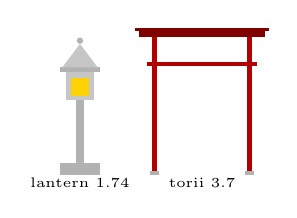
\begin{tikzpicture}[scale=1.0]
\begin{scope}
\fill[gray!60] (-0.25,0) rectangle (0.25,0.15);
\fill[gray!60] (-0.05,0.15) rectangle (0.05,0.95);
\fill[gray!45] (-0.175,0.95) rectangle (0.175,1.30);
\fill[yellow!70!orange] (-0.12,1.0) rectangle (0.12,1.22);
\fill[gray!60] (-0.25,1.30) rectangle (0.25,1.36);
\fill[gray!45] (-0.225,1.36)--(0.225,1.36)--(0,1.66)--cycle;
\fill[gray!60] (0,1.70) circle (0.04);
\node[lbl,below] at (0,0) {lantern 1.74};
\end{scope}
\begin{scope}[xshift=1.55cm,scale=0.5]
\foreach \x in {-1.2,1.2} {\fill[red!70!black] (\x-0.06,0.1) rectangle (\x+0.06,3.5); \fill[gray!60] (\x-0.11,0) rectangle (\x+0.11,0.1);}
\fill[red!50!black] (-1.6,3.5) rectangle (1.6,3.65);
\fill[red!50!black] (-1.7,3.65) rectangle (1.7,3.73);
\fill[red!70!black] (-1.4,2.75) rectangle (1.4,2.85);
\node[lbl,below] at (0,0) {torii 3.7};
\end{scope}
\end{tikzpicture}}{%
\parts{Lantern base, pillar & box, cylinder & base $0.5\times0.15$; pillar \O0.10, height 0.8\\
Light chamber & 2 boxes & $0.35^3$ at $y=0.95$; inner box glows $(0.70,0.45,0.12)$ at night\\
Cap, finial & box, cone, sphere & cap $0.5\times0.06$; cone \O0.45, height 0.30; finial at $y=1.66$\\
Torii pillars & 2 cylinders & \O0.12, height 3.5 at $x=\pm1.2$, on stone bases \O0.22\\
Kasagi, nuki & 3 boxes & top beam $3.2\times0.15$ + cap $3.4\times0.08$ at $y=3.5$; lower beam $2.8\times0.10$ at $y=2.8$; wedges\\}}

\subsection{Neighbouring houses}
\objcard{House type 1 (\code{drawJapaneseHouse}), front elevation}{%
\begin{tikzpicture}[scale=0.55]
\fill[orange!10] (-2,0.1) rectangle (2,2.8);
\foreach \x in {-2,2} \fill[brown!40!black] (\x-0.08,0.1) rectangle (\x+0.08,2.8);
\fill[gray!70!black] (-2.7,2.8) rectangle (2.7,2.86);
\fill[brown!60!black] (-2.7,2.86)--(2.7,2.86)--(2.45,4.26)--(-2.45,4.26)--cycle;
\foreach \x in {-0.8,0.8} {\fill[white,draw=brown!50!black] (\x-0.6,1.0) rectangle (\x+0.6,2.0); \draw[brown!50!black] (\x,1.0)--(\x,2.0) (\x-0.6,1.5)--(\x+0.6,1.5);}
\fill[brown!60] (-0.35,0.1) rectangle (0.35,1.9);
\fill[brown!40] (-2.15,0.25) rectangle (2.15,0.31);
\foreach \x in {-1.4,-0.5,0.5,1.4} \fill[red!80!black] (\x,2.2) ellipse (0.12 and 0.16);
\draw[dim] (-2,-0.25)--(2,-0.25) node[midway,below,lbl]{4.0};
\draw[dim] (2.9,0)--(2.9,2.8) node[midway,right,lbl]{2.8};
\end{tikzpicture}}{%
\parts{Walls & 4 textured boxes & $4.0\times3.5$, height 2.8, plaster texture\\
Frame & boxes & corner posts $0.16$, top beams, side mid-beams at $y=1.4$, foundation stones\\
Front & 2 shoji windows, box & windows $1.2\times1.0$ at $x=\pm0.8$, $y=1.5$; door $0.7\times1.8$ with a knob\\
Veranda & textured box, posts & deck $(w{+}0.3)\times0.06\times1.1$ at $y=0.28$\\
Roof & eave box, textured wedge & $(w{+}1.4)\times1.4\times(d{+}2.4)$, roof-tile texture, ridge cap, 8 rafters under each eave\\
Lanterns & 4 ellipsoids & red, emissive at night, at $y=2.2$; warm light spill on the ground\\}}

\objcard{House type 2 (\code{drawJapaneseHouse2}), front elevation}{%
\begin{tikzpicture}[scale=0.42]
\fill[brown!40!black] (-3.1,0.35) rectangle (3.1,0.43);
\foreach \x in {-2.4,0,2.4} \fill[brown!40!black] (\x-0.07,0) rectangle (\x+0.07,0.35);
\foreach \i in {0,1,2,3} {\fill[white,draw=brown!50!black] (-3+1.5*\i+0.04,0.48) rectangle (-3+1.5*\i+1.46,2.37); \draw[brown!50!black] (-3+1.5*\i+0.75,0.48)--(-3+1.5*\i+0.75,2.37);}
\fill[brown!40] (3.0,0.35) rectangle (4.2,0.41);
\fill[gray!70!black] (-3.84,2.4) rectangle (4.56,2.45);
\fill[brown!60!black] (-3.84,2.45)--(4.56,2.45)--(4.3,3.55)--(-3.58,3.55)--cycle;
\foreach \x in {-1.5,1.5} \fill[red!80!black] (\x,2.1) ellipse (0.12 and 0.16);
\draw[dim] (-3,-0.3)--(3,-0.3) node[midway,below,lbl]{6.0};
\node[lbl,below] at (3.6,0.3) {porch};
\end{tikzpicture}}{%
\parts{Raised floor & posts, textured box & 6 posts $0.14\times0.35$ on stones; floor $6.2\times0.08\times3.7$\\
Walls & textured boxes & plaster back wall, dark-wood side panels, a half right wall (side entrance)\\
Front & 4 shoji panels & each $1.42\times1.84$, with divider posts\\
Side porch & box, posts & $1.2$ wide on the right, with its own posts and stones\\
Roof & wedge & $8.4\times1.1\times4.7$, offset 0.36 to cover the porch; 10 rafters; 2 red lanterns\\}
Ten houses (5 of each type) line both sides of the street; each one is skipped when it is outside the view frustum.}

\subsection{Characters and animals}
\objcard{Cyclist (\code{drawBicycle}), scale 1.4}{%
\begin{tikzpicture}[scale=2.1]
\foreach \x in {-0.52,0.52} {\draw[thick] (\x,0.33) circle (0.33); \draw[gray] (\x,0.33) circle (0.26); \foreach \a in {0,60,120} \draw[gray,thin] ($(\x,0.33)+(\a:0.26)$)--($(\x,0.33)+(\a+180:0.26)$);}
\draw[red!70!black,thick] (-0.02,0.30)--(-0.20,0.86)--(0.38,0.84)--(-0.02,0.30) (-0.52,0.33)--(-0.02,0.30) (-0.52,0.33)--(-0.20,0.86) (0.52,0.33)--(0.38,0.84)--(0.34,1.02);
\draw[dashed,gray] (-0.02,0.30) circle (0.17);
\fill[black] (-0.33,0.86) rectangle (-0.11,0.90);
\draw[blue!50!black,line width=2.5pt] (-0.22,0.98)--(0.04,1.46);
\draw[blue!30!black,line width=1.5pt] (-0.22,0.98)--(0.116,0.65)--(0.065,0.183);
\fill[orange!30] (0.10,1.64) circle (0.10);
\draw[blue!50!black,line width=1.2pt] (0.04,1.42)--(0.34,1.02);
\fill (0.116,0.65) circle (0.02) node[right,lbl]{knee (IK)};
\fill (-0.22,0.98) circle (0.02) node[left,lbl]{hip};
\node[lbl,below] at (0.065,0.12) {pedal};
\end{tikzpicture}}{%
\parts{Wheels (2) & torus, torus, 6 tubes, sphere & tyre radius 0.33, rim 0.26, spokes, hub; turned $\theta=-d/(rS)$\\
Frame & 7 tubes (\code{limb}) & between rear hub, bottom bracket $(-0.02,0.30)$, seat $(-0.20,0.86)$, head tube $(0.38,0.84)$, front hub\\
Cranks, pedals & tubes, boxes & length 0.17, angle $0.55\,d/(rS)$, $180^\circ$ apart\\
Rider & cylinder, spheres & torso hip $(-0.22,0.98)\to$ shoulder $(0.04,1.46)$; head at $y=1.64$\\
Legs & 2+2 tubes & bones $0.47+0.47$, knee from two-bone IK (law of cosines)\\
Lights & spheres, triangle & headlight emissive at night + additive road beam; red reflector\\}}

\objcard{Walking person (\code{drawWalkingPerson})}{%
\begin{tikzpicture}[scale=1.65]
\draw[gray!40!blue,line width=2pt] (0,0.92)--(0.13,0.48)--(0.02,0.06);
\draw[gray!60!blue,line width=2pt] (0,0.92)--(-0.12,0.48)--(-0.26,0.08);
\fill[black!70] (0.0,0.02) rectangle (0.14,0.08); \fill[black!70] (-0.30,0.04) rectangle (-0.16,0.10);
\fill[red!60!black] (-0.15,0.96) rectangle (0.15,1.42);
\draw[red!50!black,line width=1.6pt] (0,1.40)--(-0.1,1.12)--(-0.04,0.86);
\fill[orange!30] (0,1.69) circle (0.11); \fill[black!80] (-0.02,1.76) ellipse (0.11 and 0.06);
\foreach \p in {(0,0.92),(0.13,0.48),(-0.12,0.48),(0,1.40),(-0.1,1.12)} \fill[ramen] \p circle (0.022);
\node[lbl,right] at (0.15,0.48) {knee};
\node[lbl,right] at (0.05,0.92) {hip $\pm28^\circ$};
\node[lbl,left] at (-0.12,1.12) {elbow};
\draw[dim] (0.42,0)--(0.42,1.8) node[midway,right,lbl]{1.8};
\end{tikzpicture}}{%
\parts{Legs & 2+2 tubes, shoes & thigh 0.46, shin 0.44 from hip $y=0.92$; thigh $\pm28^\circ\sin\varphi$, knee $35^\circ\max(0,\sin(\varphi+\varphi_0))$\\
Hips, torso & box, frustum & torso radius $0.15\to0.18$, height 0.44; shoulders an ellipsoid\\
Arms & 2+2 tubes, hands & upper arm 0.30, forearm 0.27, swing $-0.8\times$ leg angle, elbow $15^\circ$\\
Head & spheres & face $0.21\times0.24$, hair cap, neck tube\\}
A joint hierarchy: every \code{glRotatef} at a joint moves everything below it.}

\objcard{Shop cat (\code{drawWalkingCat}, \code{drawCatHead}), scale 1.8}{%
\begin{tikzpicture}[scale=3.0]
\foreach \x/\s in {0.15/0.04,-0.15/-0.03} \draw[orange!70!brown,line width=2pt] (\x,0.20)--(\x+\s,0.0);
\fill[orange!70!brown] (0,0.24) ellipse (0.23 and 0.085);
\fill[orange!40!brown] (0.02,0.29) ellipse (0.17 and 0.04);
\fill[orange!70!brown] (0.27,0.34) circle (0.075);
\fill[orange!70!brown] (0.24,0.39)--(0.26,0.46)--(0.29,0.40)--cycle; \fill[orange!70!brown] (0.29,0.40)--(0.31,0.46)--(0.33,0.39)--cycle;
\fill[green!60!black] (0.32,0.355) circle (0.012);
\draw[orange!70!brown,line width=2pt] (-0.22,0.26) .. controls (-0.30,0.32) and (-0.30,0.44) .. (-0.32,0.50);
\draw[dim] (-0.23,-0.06)--(0.35,-0.06) node[midway,below,lbl]{0.58 (local)};
\end{tikzpicture}}{%
\parts{Body & 2 ellipsoids & $0.46\times0.17\times0.17$ at $y=0.24$ and a darker back stripe\\
Legs & 4 tubes, paws & from $y=0.20$ at $(\pm0.15,\pm0.06)$; swing $0.06\sin(\varphi+\varphi_i)$, lift $0.025\max(0,\cos(\cdot))$\\
Head & ellipsoids, cones & face, crown, cream muzzle, pink nose, ears (cones), green or closed eyes\\
Tail & 5 (walk) / 7 (sit) tubes & sways $0.06u\sin(2.5t+1.5u)$; curled round the paws when sitting\\}
A state machine changes the pose: walking, turning, sitting and washing its face (Section~\ref{sec:anim}).}

\objcard{Duck (\code{drawDuck}), two on the lake}{%
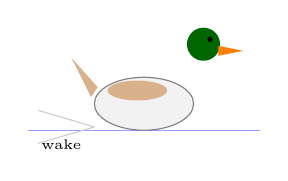
\begin{tikzpicture}[scale=4.2]
\draw[blue!40] (-0.35,0)--(0.35,0);
\fill[gray!10,draw=gray] (0,0.08) ellipse (0.15 and 0.08);
\fill[brown!60] (-0.02,0.12) ellipse (0.09 and 0.03);
\fill[green!40!black] (0.18,0.26) circle (0.05);
\fill[orange] (0.225,0.255)--(0.30,0.24)--(0.225,0.225)--cycle;
\fill[brown!60] (-0.14,0.13)--(-0.22,0.22)--(-0.16,0.10)--cycle;
\fill (0.20,0.275) circle (0.008);
\draw[gray!40] (-0.15,0.01)--(-0.32,0.06) (-0.15,0.01)--(-0.32,-0.04);
\node[lbl,below] at (-0.25,-0.02) {wake};
\end{tikzpicture}}{%
\parts{Body & ellipsoid & $0.22\times0.16\times0.30$, white\\
Wings, tail & ellipsoids, cone & brown patches tilted $\pm15^\circ$; tail cone tilted $45^\circ$\\
Head, beak, eyes & sphere, cone, spheres & green head \O0.10 at $(0,0.26,0.18)$; orange beak; black eyes\\
Wake & 2 triangles & translucent V behind the duck (alpha 0.18)\\}
It swims on the circle $(3.5\cos0.4t,\,3.5\sin0.4t)$, turned to face its direction, and bobs $0.03\sin2t$.}

\subsection{Trees and the bridge}
\objcard{Cherry blossom tree (\code{buildCherryVariant}, \code{growBranch})}{%
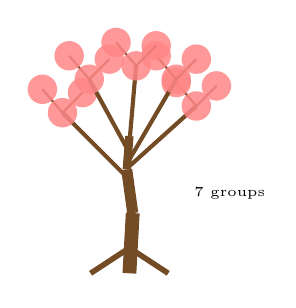
\begin{tikzpicture}[scale=0.85]
\draw[brown!60!black,line width=5pt] (0,0)--(0.05,0.9);
\draw[brown!60!black,line width=4pt] (0.05,0.9)--(-0.04,1.55);
\draw[brown!60!black,line width=3pt] (-0.04,1.55)--(0,2.05);
\foreach \a in {-1,1} \draw[brown!60!black,line width=2pt] (0,0.38)--(\a*0.58,0);
\foreach \x/\y/\ex/\ey in {0/1.4/-1.0/2.4, 0/1.6/1.0/2.5, 0/1.8/-0.6/2.9, 0/1.7/0.7/2.9, 0/1.95/0.1/3.1}
  {\draw[brown!60!black,line width=1.5pt] (\x,\y)--(\ex,\ey);
   \draw[brown!60!black,line width=0.8pt] (\ex,\ey)--(\ex-0.3,\ey+0.35) (\ex,\ey)--(\ex+0.3,\ey+0.3);
   \foreach \dx/\dy in {-0.3/0.35,0.3/0.3,0/0} \fill[pink!70!red,opacity=0.85] (\ex+\dx,\ey+\dy) circle (0.22);}
\node[lbl] at (1.5,1.2) {7 groups};
\end{tikzpicture}}{%
\parts{Trunk & 3 tapered tubes & $(0,0)\to(0.05,0.9)\to(-0.04,1.55)\to(0,2.05)$, radius $0.27\to0.12$\\
Roots & 5 tubes & from $y=0.38$ to radius 0.58 on the ground, $72^\circ$ apart\\
Branch groups & 7 recursive branches & 6 around the trunk from $y=1.3$--$1.95$, $36^\circ$--$66^\circ$ from vertical, length 1.25--1.5, plus a top leader\\
Recursion & \code{growBranch} & level 1: 3 children, then 2; length $\times0.6$, radius $\times0.55$; 3 levels\\
Blossoms & petal clusters & cluster size $0.40/0.34/0.29$ per level; 14 falling petals, carpet of 110\\}
Each of the 7 groups is a display list that sways about its own pivot.}

\objcard{Japanese pine (\code{buildPineVariant})}{%
\begin{tikzpicture}[scale=0.72]
\draw[brown!50!black,line width=4pt] (0,0)--(0.03,1.4)--(-0.02,3.3);
\foreach \y/\R/\d in {0.85/1.27/0.5, 1.36/1.077/0.455, 1.87/0.884/0.41, 2.38/0.690/0.365, 2.89/0.497/0.32, 3.40/0.304/0.275}
  {\fill[green!40!black] (-\R,\y-\d)--(-\R*0.7,\y-\d+0.08)--(-\R*0.5,\y-\d-0.04)--(0,\y+0.22)--(\R*0.5,\y-\d-0.04)--(\R*0.7,\y-\d+0.08)--(\R,\y-\d)--cycle;}
\fill[green!50!black] (-0.14,3.25)--(0.14,3.25)--(0,3.75)--cycle;
\draw[dim] (1.5,0)--(1.5,3.75) node[midway,right,lbl]{3.75};
\end{tikzpicture}}{%
\parts{Trunk & 2 tubes, 4 roots & $(0,0)\to(0.03,1.4)\to(-0.02,3.3)$, radius $0.17\to0.04$\\
Skirts & 6 tiers $\times$ 2 fans & tier $t$: $y=0.85+2.55u$, $R=1.15(1-0.84u)+0.12$, droop $0.5(1-0.45u)$ ($u=t/5$); 18 jagged points, light centre, dark rim\\
Spire & triangle fan & from $y=3.25$ to $3.75$\\}
The whole crown sways by $1.3^\circ$ times the breeze function.}

\objcard{Arched footbridge (\code{drawBridge}) over the lake}{%
\begin{tikzpicture}[scale=0.3]
\draw[brown!50!black,line width=2.5pt,domain=-8.5:8.5,samples=40] plot (\x,{0.6*cos(\x*180/17)});
\foreach \i in {0,...,8} {\pgfmathsetmacro{\z}{-8.5+\i*17/8}\pgfmathsetmacro{\h}{(\i==0||\i==8)?1.4:0.8}
  \draw[red!70!black,line width=1.5pt] (\z,{0.6*cos(\z*180/17)})--(\z,{0.6*cos(\z*180/17)+\h});}
\draw[gray!30!black,domain=-8.5:8.5,samples=30] plot (\x,{0.6*cos(\x*180/17)+0.65});
\draw[gray!30!black,domain=-8.5:8.5,samples=30] plot (\x,{0.6*cos(\x*180/17)+0.35});
\draw[yellow!60!orange,dashed,domain=0:1,samples=20] plot ({-8.5+17*\x},{1.46-0.4*sin(\x*180)});
\draw[dim] (-8.5,-0.6)--(8.5,-0.6) node[midway,below,lbl]{17};
\end{tikzpicture}}{%
\parts{Deck & 34 boxes & planks $1.6$ wide on the arch $y=0.6\cos(\pi z/17)$\\
Edges & 68 boxes & metal trim under both sides (conductive specular)\\
Posts & 18 boxes, spheres & red, 0.8 tall (corners 1.4), red ball finials\\
Rails & 32 tilted boxes & two rails at $+0.35$ and $+0.65$ following the arch\\
String lights & wire, 18 spheres & sag $-0.4\sin(\pi t)$ between the corner posts; emissive at night\\}}
